\hyphenation{ma-te-rials}
%%%%%%%%%%%%%%%%%%%%% Introduction %%%%%%%%%%%%%%%%%



\chapter{Introduction}
\label{ch:intro}

This chapter describes the development of particle physics following the historical order of how particles were discovered and parts of the Standard Model (SM) were constructed. 

\section{``All things are made of atoms''}

\indent The SM is the theory of particles and their interactions that was built during many decades of intense experimental and theoretical work. Particles in this theory are elementary and have no internal structure, meaning they cannot be divided further. This idea of point-like particles is crucial since it reflects the goal of particle physics to find and describe the smallest and the most fundamental scale at which nature works. For the last several decades the SM has been the most tested theory of elementary particles and forces that is presently generally accepted by the whole physics community. 

Formally, all SM elementary particles are split into two classes: fermions and bosons. Particles with a half-integer spin 1/2 (quarks and leptons) are called fermions since they obey Fermi-Dirac statistics ~\cite{statmech}. The other class of particles is bosons. They are force carriers, have an integer spin, and are characterised by the Bose-Einstein statistics. A rigorous mathematical description of the SM will be given in the next chapter. 

The quest for the smallest scale and the theory that would describe this scale were the key ideas that ultimately led to the development of the SM.
However, particle physics did not start with quarks. Physicists were discovering more and more fundamental scales over the course of hundreds of years; starting first with our macroscopic world that is made of atoms (the atomic theory). Richard Feynman, a Physics Nobel Prize winner, %whom I consider one of the brightest physicists who has ever lived on Earth, 
once summarised in a single phrase what he believed to be the most important fact about the world around us: ``all things are made of atoms'' \cite{Feynman_atoms}. Feynman himself was the father of quantum electrodynamics, and in this simple statement - delivered originally to Caltech students and now known to public through his series of physics books - he decided not to go into quantum mechanics principles and instead illustrated at the rather highly abstract that everything can be made of a set of smaller particles, praising the importance of the atomic theory. 


Today the physics community knows that atoms are not elementary particles. Instead, they have heavy nuclei and light electrons ``orbiting'' around the nucleus on the electron shells. The nucleus is positively charged proportionally to the number of protons it contains. To provide the stability of the nuclei of the heavy atoms our world also needs neutrons, which have no electric charge. %A free neutron decays in about 15 minutes, while the proton is stable, as far as we know from the experiments, and only in some exotic %Beyond the Standard Model (BSM) theories it is hypothesised that the proton lifetime is finite. However, the estimate of the proton lifetime is a value that is larger than the age of our Universe and is at least $10^{30}$ years \cite{DIMOPOULOS1982133}. 
Going to an even smaller scale, it is now known that protons and neutrons are not elementary; rather, they are composed of point-like constituents that are called quarks (see Figure \ref{atom_structure}). 

\begin{figure}[H]
  \centering
    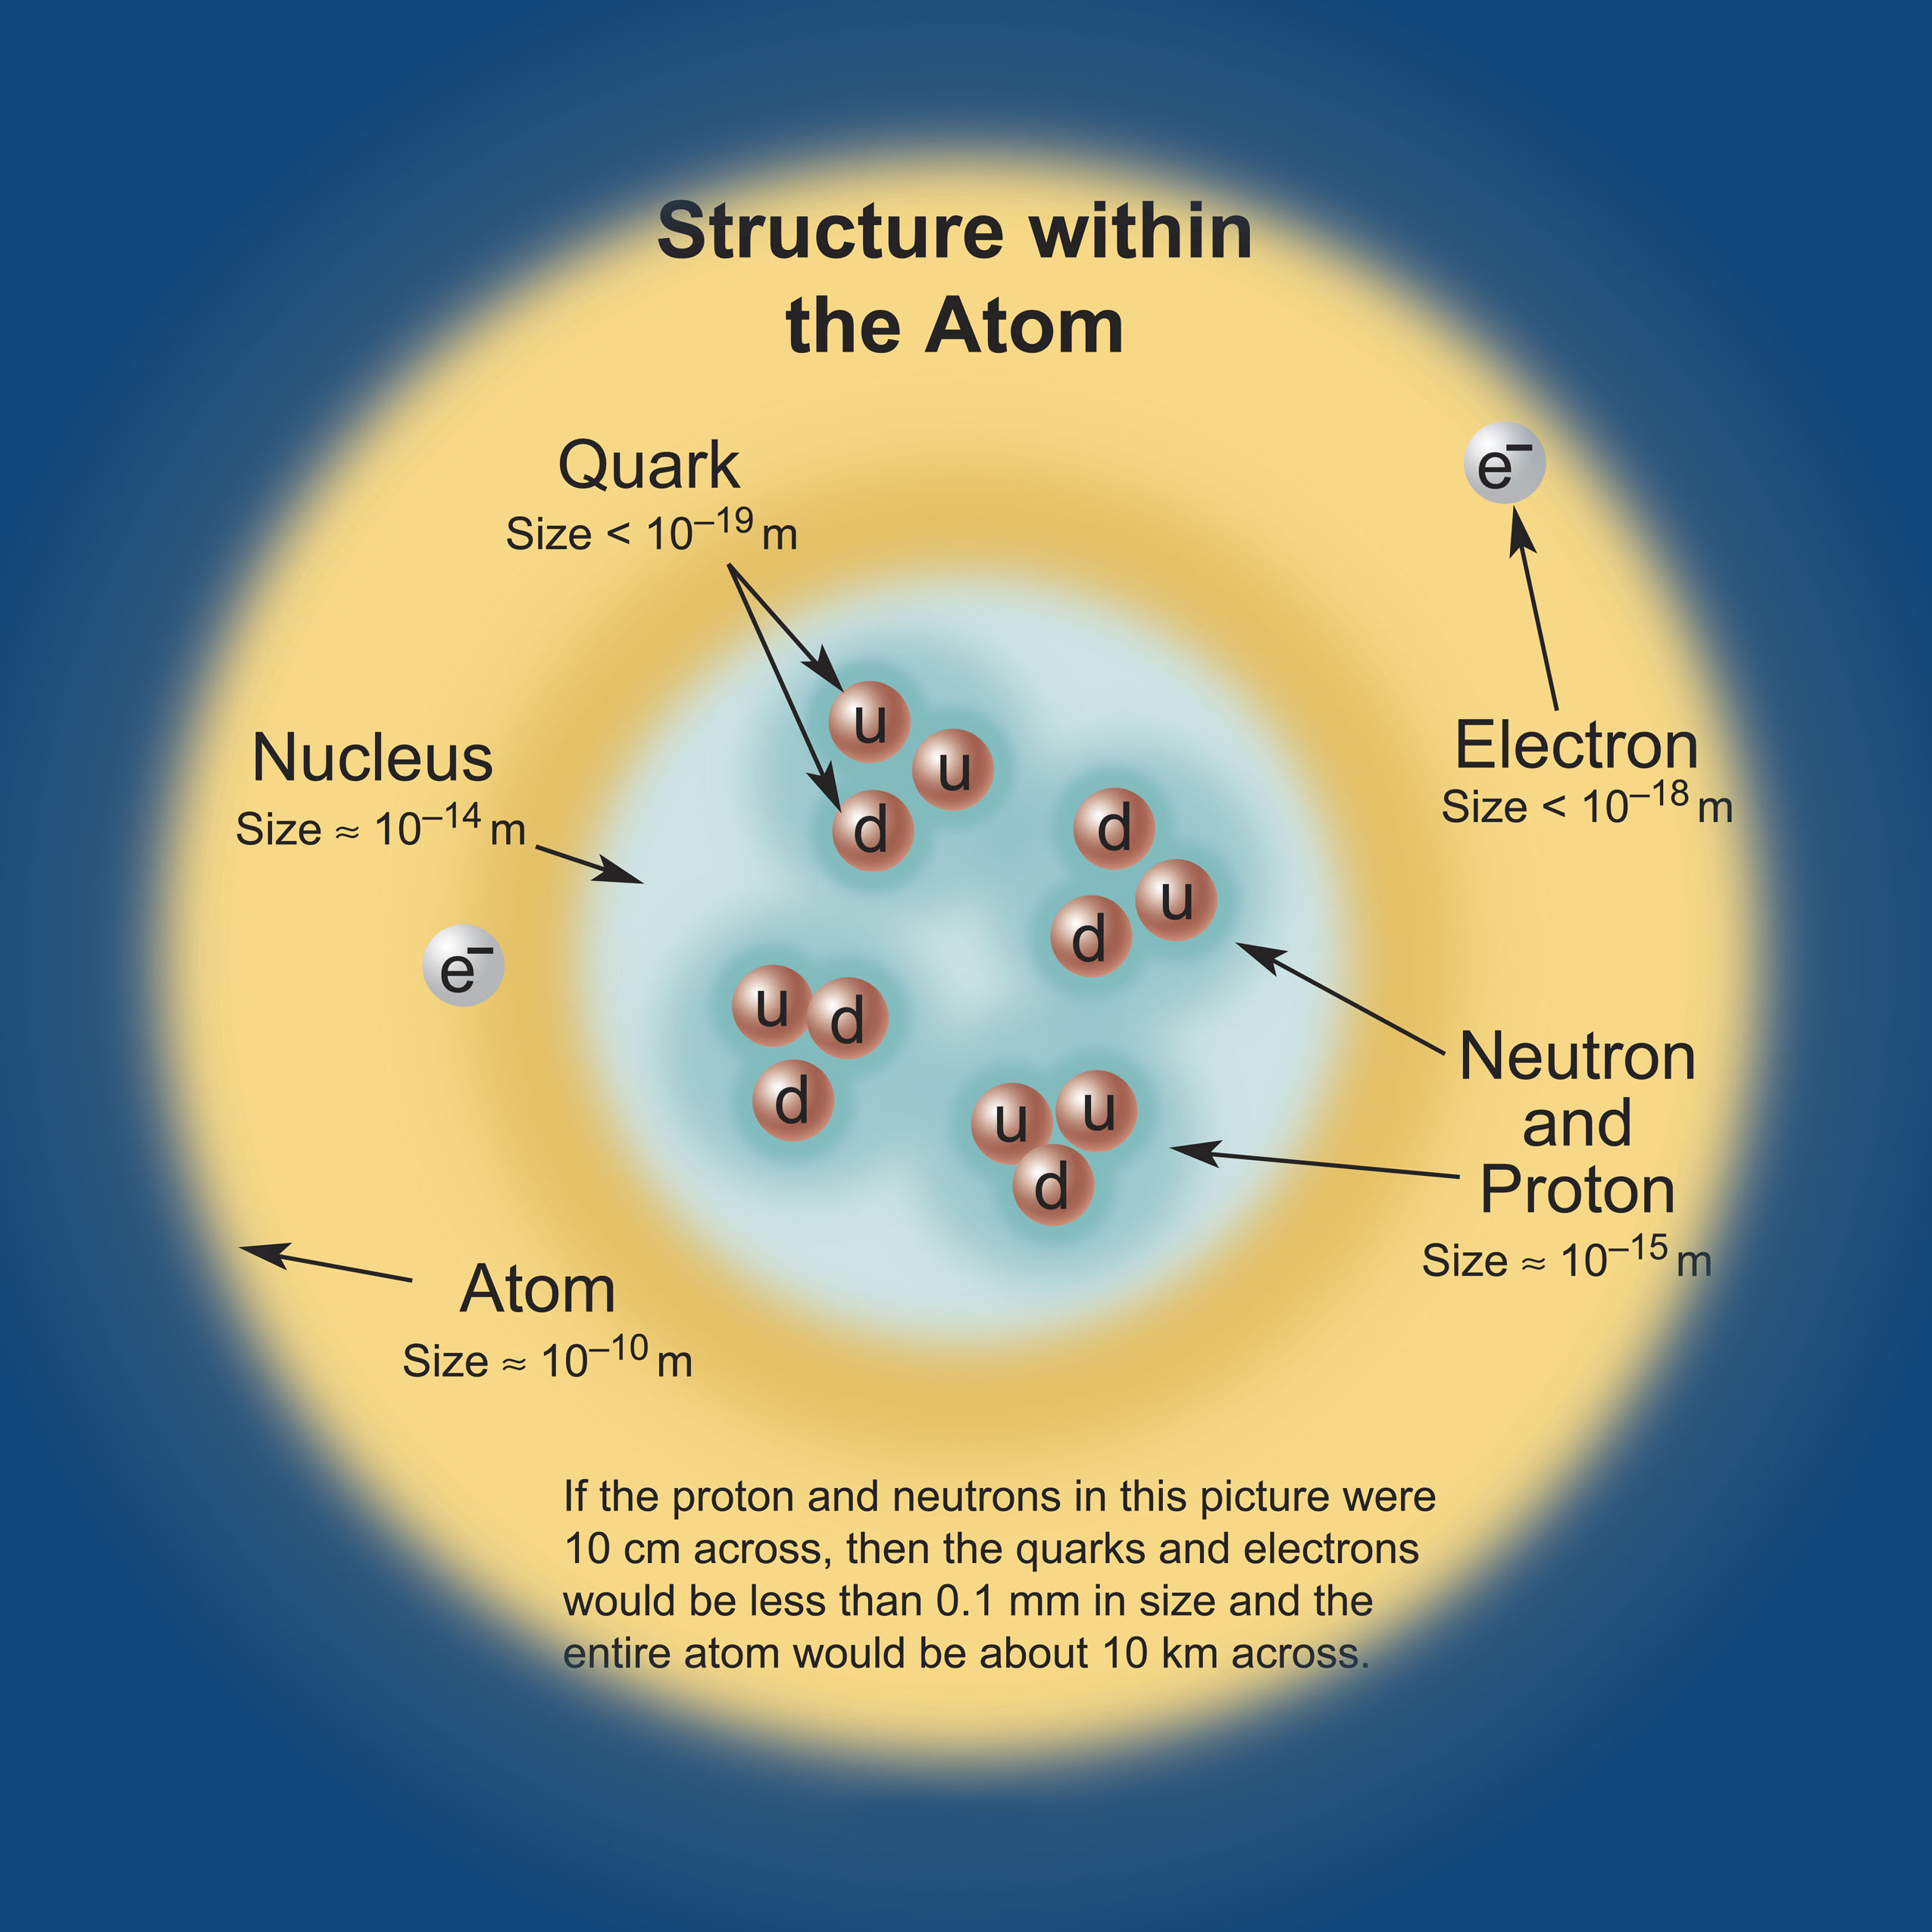
\includegraphics[width=0.70\textwidth]{atom_structure}
    \caption[The structure of an atom]{The structure of an atom. Approximate scale values are indicated.}
    \label{atom_structure}
\end{figure}

Quarks were proposed by Gell-Mann and also by Zweig to explain periodicity in properties of observed subatomic particles  \cite{griffiths_hep}. Quarks are arranged in three families or three generations of doublets. A doublet is a mathematical construct that is used to describe a two-value system. For example, in the design of Gell-Mann and Zweig, each quark doublet in their theory is a two quark system that has an ``up'' quark with electric charge $+1/3$ and a ``down'' quark with charge $-2/3$. For antiquarks, the signs of the charges are reversed. 

The physics world before Gell-Mann and Zweig got used to the fact that particles have integer charges due to an enormous number of observations. The fact that the quark charge values were fractional was so revolutionary to Gell-Mann that he decided not to publish his article in a highly prestigious journal but, expecting a rejection, decided to go with a second tier one \cite{griffiths_hep}. However, with time, out of all the theories that were trying to explain the difference in masses of observed hadrons it was the hypothesis of Gell-Mann and Zweig that was not disproven. Now, the quark theory is generally accepted and is one of the key elements of the SM. 

The SM includes six different types of quarks: up, down, charm, strange, top, and bottom. To distinguish one quark from another there is a ``flavor'' number assigned to them. For instance, a charm quark has $+1$ unit of ``charmness'', while a strange quark has $-1$ unit of ``strangeness''. All of the other flavor fields are zero for a given quark. 

Another important characteristic of quarks was revealed at the $e^+e^-$ colliders when physicists compared production rates of muons and hadrons. At that time it was assumed that quarks differ only by flavor, therefore, when comparing the calculations with the data, the theory was off by a factor of three. This was the motivation to introduce a new quark property - a ``colour'' - and thus three quark colours: green, blue, and red. 

\section{A brief history of particle physics}

The electron is the first particle that was observed in a particle physics experiment. The electron belongs to a family of leptons. A lepton is an elementary particle with a spin 1/2. Charged leptons participate in all but strong interactions. Neutral leptons or neutrinos - interact only weakly, which will be discussed in more detail later in this chapter. The electron was discovered by Thompson \cite{Davis:1989898} in 1897 when he was studying the properties of a cathode ray. Due to this discovery, that year may be considered the beginning of an era of a particle physics: dozens of particles were discovered in the next decades. In 1936, another lepton was observed, the muon \cite{Piccioni1996}, in an experiment of Anderson and Neddermeyer who studied cosmic radiation. In essence, a muon has very similar characteristics to those of an electron, but its mass is 207 times heavier. No explanation for this mass difference exists in the SM \footnote{According to mathematical physicist Carl Bender, who is known for advances in perturbative Quantum Field Theory (QFT) and demonstration of the importance of parity-time (PT) symmetry in quantum theory, there is a story that Feynman was able to derive the mass of the muon starting with the mass of an electron, but the world has never seen that calculation published \cite{Bender} }. 


Leptons are also arranged in generations, analogously to quark families. Each generation is a doublet that consists of a charged lepton (electron, muon or tau) with the charge $-1$ and a neutral lepton (corresponding electron, muon, or a tau neutrino). Electron and muon neutrinos had been directly detected in experiments of 1956 and 1962, respectively. 
The existence of the electron neutrino is deduced from the violation of the conservation of energy in a beta decay. The muon neutrino \cite{PhysRevLett.9.36} was discovered by Schwartz, Lederman, and Steinberger during an experiment with a pion beam where leptons from the pion decays arrived to the an aluminum spark chamber after passing a steel wall. Fifty-one events of interest had been observed after running the experiment for several months.
Those events could not be initiated by electron neutrinos, since they will interact with the metal and produce electrons. The presence of narrow muon tracks in the chamber in each event, hence muons, was a clear indication that those neutrinos were of a different kind - they were muon neutrinos. Finally, a tau lepton and a tau neutrino were discovered in 1975 and 2000 correspondingly \cite{PhysRevLett.35.1489, Kodama:2000mp}. With that, all three families of the SM leptons were observed: a long-awaited tau neutrino, which decades ago was theoretically predicted to exist, was finally discovered experimentally. In a like manner to families of quarks, lepton masses grow with each generation, where a tau from the third generation is the heaviest lepton. To classify leptons of different families the lepton numbers were reserved: 1 unit of electron number to an electron and an electron neutrino, 1 unit of muon number to a muon and a muon neutrino, and 1 unit of tau number to a tau and a tau neutrino.



\section{Fundamental forces}

In nature there are four fundamental forces: gravitational, weak, electromagnetic, and strong forces. 
%At the fundamental level the world is made of quarks and leptons. And there must be rules, at least we expect them to exist, which explain how quarks/leptons interact. These rules are referred to as fundamental forces of nature. 
This thesis will classify all four forces \cite{wolfram} in terms of the relative strength, the range that they can cover, the spin of the mediator, and whether the force (when appplicable) is attractive, repulsive, or both. This should be taken critically, since this is quite an ambiguous categorisation. It has a deep pedagogical meaning, though, because it helps to illustrate in which regime each of the forces is dominant. According to the world known mathematical physicist Carl Bender, this is of great importance since it is one of the main approaches to solving physics problems: to know which effects are the dominant and which are sub-dominant. This helps to justify what effect can be neglected and what approximation can be used. Thus, it allows the possibility to do calculations for problems where closed-form solutions do not exists, which is almost all the complex phenomena around us \cite{Bender}. 


The first force on our list of forces is the gravitational force. This force governs the Universe at the macroscopic level of astronomic objects: planets, solar systems, galaxies. The first theory of gravity was formulated by Newton \cite{Chandrasekhar:1187874}. Einstein later developed a new theory of gravity (GR). The key difference is that the Newtonian gravity had several ``absolutes'' that GR does not have: absolute time and space, a preferred separation of spacetime into time and spatial parts, absolute simultaneity, etc. 
%and a curved connection that is not the special one derived from a spacetime metric (Christoffel symbols.
\cite{MTW_gravity}. Butterworth gives a good historical perspective in \cite{Gutfreund:1980674}. 

It is worth noting that the gravitational force is not included in the SM. Attempts are ongoing to expand the SM, e.g., adding the graviton as a mediator, but no real success so far has been achieved to create a renormalizable theory that would combine both the SM and gravity \cite{butterworth2014smashing}. Surprisingly, gravity is the weakest force; the only reason why the motion of planets and galaxies is governed by gravity is because those are gigantic objects. Gravity effects become the dominant ones at the macroscopic scale because of an enormous number of particles involved in the interaction. If the strength of the strongest force, which is the strong force, is set to 1, then the strength of the gravity will be about $10^{-41}$ \cite{wolfram}. In a modern High Energy Physics (HEP) language, which uses the term ``coupling constant'' to quantify the  strength of the interaction between two elementary particles for a given force, a gravitational coupling constant can be considered as a constant characterizing the gravitational attraction between, e.g., a pair of electrons. In this case, $\alpha_G \approx 10^{-39} $. It is contemplated that the gravity mediator, if it exists, would have a charge of zero, zero mass, spin 2, and should be a stable particle. From the observations, the gravitational force is of the infinite range and its nature is purely attractive, while the other three forces can exhibit both an attractive and a repulsive behaviour. Einstein's general relativity theory, though not a quantum theory, is the only working theory of gravity as of now.

The next force, the weak force, is mediated by a charged W (charge +1/-1) boson or a neutral Z boson, thus giving name to charged and neutral weak interactions correspondingly. All SM fermions, quarks and leptons,  experience the weak force. %For leptons, it is worth mentioning here that neutral leptons have no charge, thus will not participate in the electromagnetic interactions, and all leptons have no color charge, so they feel no strong force \cite{griffiths_hep}. 
All three weak bosons ($W^+$, $W^-$, and Z) have spin 1.
The relative strength of the weak force is $10^{-16}$ ($\alpha_W \approx 10^{-6}$) and the range of applicability is $10^{-3}$ fm. The range of the force can be well approximated by the expression $\frac{\hbar}{mc}$ \cite{Zee_qft}, where $m$ is the mass of the mediator or of the parent particle that decays. The range of applicability of the weak force is relatively short since the bosons are quite massive: $m_{W^\pm} = 80. 385$ GeV and $m_{Z}=91.189$ GeV \footnote{GeV is the unit of the ``natural system of units'', in which $\hbar = c = 1$. This natural system of units is very popular in the high-energy physics and is widely used in this thesis. Adoption of this system simplifies how many equations look. Using the natural system of units \cite{Cottingham:1026625}, masses, momenta, and energies are measured in electronvolts (eV), with GeV ($10^9 $~eV) and TeV ($10^{12}$~eV) being the most popular units in a modern high-energy physics due to the energy regimes involved }. 


Let us think of an interaction process as initial state particles interacting at the interaction vertex and producing final state particles. For our purposes, we follow this simplified description. In practice, HEP calculations are done using the Feynman diagram approach \cite{feynman_diagrams}. In this approach, a set of rules and conventions is developed to substitute the mathematics of a given process by the corresponding diagram. In the Feynman diagram formulation of the quantum mechanics, each vertex corresponds to an interaction term in the Lagrangian \footnote{The Lagrangian of the SM will be discussed in the next chapter} describing a given process, where both the energy and the momentum of interacting particles have to be conserved. For the details about the actual principles behind the approach of Feynman diagrams, we refer the reader to \cite{griffiths_hep, Halzen:100339, Zee_qft}. In our simplified diagrammatic representation, charged weak interactions are interesting due to the fact that a primitive interaction vertex can be thought of as a point where a charged lepton is converted to a neutral lepton or vice versa. A good example is a muon decay, which is a conversion of the muon to a muon neutrino with the help of the W boson, which further decays to an electron and a corresponding electron antineutrino. %Lepton numbers are conserved during weak interactions and conversions happen only within the same family of leptons. However, c
It is worth noting that charged weak interactions do not conserve the flavor of quarks. Also, weak interactions do not conserve the generation number, e.g., members of doublets of the third and the second families can be converted into members of the lower family of quarks. This fact is reflected in the Cabibbo-Kobayashi-Maskawa (CKM) matrix \cite{pdg}. The elements of this matrix are used to quantify the strength of the flavor-changing weak interactions. Since diagonal elements of this matrix are less than one and off-diagonal elements are non-zero, the CKM matrix represents a mismatch of quantum states of quarks when they propagate freely and when they take part in the weak interactions. In other words, the CKM matrix with non-zero off-diagonal elements means cross-generation interactions are allowed.% and this is the information that the CKM matrix quantifies.

\begin{equation}
\small
\begin{pmatrix}
|V_{ud}| & |V_{us}| & |V_{ub}| \\
|V_{cd}| & |V_{cs}| & |V_{cb}| \\
|V_{td}| & |V_{ts}| & |V_{tb}|
\end{pmatrix} = \begin{pmatrix}
0.97427 \pm 0.00015 & 0.22534 \pm 0.00065 & 0.00351^{+0.00015}_{-0.00014} \\
0.22520 \pm 0.00065 & 0.97344 \pm 0.00016 & 0.0412^{+0.0011}_{-0.0005} \\
0.00867^{+0.00029}_{-0.00031} & 0.0404^{+0.0011}_{-0.0005} & 0.999146^{+0.000021}_{-0.000046}
\end{pmatrix}.
\label{eq:ckm}
\end{equation}



The third force, the electromagnetic (EM) force, is one of the main forces that we experience in our everyday life. The reason one can sit in the chair and does not fall further down due to gravity is that electrons of the body repel electrons of the chair. The relative strength of the EM force is $10^{-3}$ ($\alpha_{EM} \approx 1/137$) and the range of applicability is infinite. A photon, as the EM force's mediator, has zero mass and spin 1. The theory that describes photon interaction with leptons and quarks is called quantum electrodynamics (QED) and was developed in 1940s and 1950s by Tomonaga, Schwinger, Feynman, and Dyson \cite{qed_fathers}. Electric charge is conserved in EM interactions and no single photon-to-fermion vertex is possible; there are always two fermions that must be involved. This force can exhibit both an attractive ($e^{\pm}$ with $e^{\mp}$) and a repulsive behaviour ($e^{\pm}$ with $e^{\pm}$). 

In the SM, several multi-boson vertices are allowed. W and Z bosons that participate in weak interactions can couple to each other, so $WWZ, WWWW$, and $WWZZ$ vertices are possible in the SM. In addition, W bosons can couple to photons, so $\gamma WW$, $\gamma WWZ$, and $WW\gamma\gamma$ vertices are allowed too. Even though Z boson is massive and photon is a massless boson, the Z boson has a neutral charge. This makes it possible that any interaction where the photon is a force carrier, can also be mediated by the Z boson, but not vice versa.


The strong force, the fourth force of nature, is the strongest known force. Gluons are the carriers of this force. They have spin 1 and are massless. The relative strength of the strong force is 1 ($\alpha_s \approx 1$) and the range of applicability is about 1 $fm$. Each gluon carries one unit of color and one unit of anticolor. There are nine types of gluons but, technically, the ninth gluon is a color invariant and would give rise to an infinite range of the strong force, which contradicts experiments. That is why modern physics assumes that in our physical world only eight gluons exist \cite{griffiths_hep, pdg}. Gluons carry color charge and, thus, can couple to each other. For several high order processes in quantum chromodynamics (QCD), 3- and 4-gluon vertices have to be introduced to restore gauge invariance and no higher order vertices are required \cite{Mangano:454171}.
 

To summarise the knowledge about the SM forces, we show the reference figure of all allowed SM particle interactions and corresponding simple vertices (Fig. \ref{SM_vertices}) in the Feynman diagram representation. 

	
\begin{figure}[H]
  \centering
    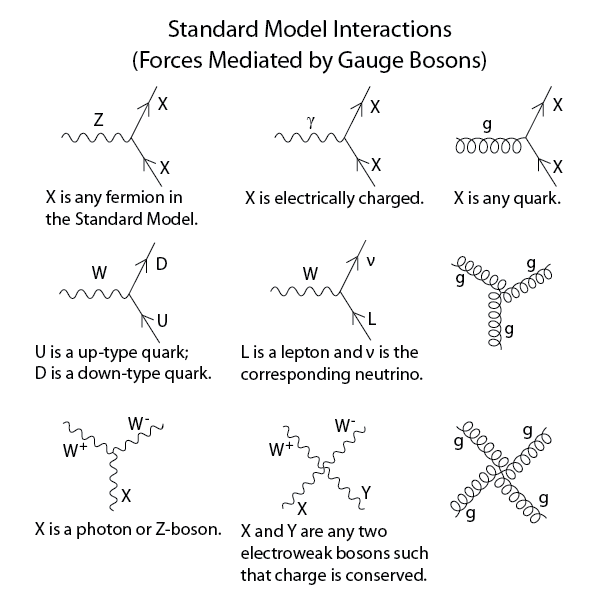
\includegraphics[width=0.70\textwidth]{Standard_Model_Feynman_Diagram_Vertices}
    \caption[All SM interaction and simple vertices]{All SM interaction and simple vertices. }
    \label{SM_vertices}
\end{figure}


\section{The Brout-Englert-Higgs mechanism}
\label{sec:BEH}
	
The description of the SM picture is not complete without mentioning the main particle - the Higgs boson - that was predicted almost 60 years ago, but was not observed until 2012 (see Fig. \ref{sm_interactions2} \cite{strassler}). After the electroweak (EW) unification by Glashow, Salam, and Weinberg \cite{Glashow:1961tr}, it was still not clear what the origin of the mass of fundamental particles is. In 1964, Robert Brout and Fran�ois Englert\cite{PhysRevLett.13.321}, Peter Higgs\cite{PhysRevLett.13.508}, Gerald Guralnik, C. Richard Hagen, and Tom Kibble \cite{PhysRevLett.13.585} (BEHGHK authors), proposed the method by which the particles can acquire mass. This technique consists of three stages and we will discuss them one-by-one:



\begin{enumerate}
\item The Brout-Englert-Higgs (BEH) mechanism
%\begin{enumerate}
%\item Nested item 1
%\item Nested item 2
%\end{enumerate}
\item The BEH field
\item The Higgs boson.
%\ldots
\end{enumerate}

The first stage, the BEH mechanism, is simply a spontaneous symmetry breaking (SSB) mechanism, which can be thought of as a mathematical trick consisting of rewriting the original scalar fields in the EW Lagrangian, rearranging equations, and requiring that the fields are real. What does this lead to? The BEH authors started with a scalar complex field and a massless vector field and after SSB obtained a single real scalar field (Higgs boson) and a massive vector field. In terms of our physical world this it what gives mass to W and Z bosons. 




The second stage is the BEH field. It exists everywhere and has been present almost since the Big Bang \cite{who_cares}. It is a property of our world. All the fundamental particles that interact with the BEH field acquire mass. Those, which do not interact directly (at the tree diagram level) have no mass and all their energy is in the form of the momentum. Such particles can travel with the speed of light. The more the particle interacts with the BEH field, the higher is the coupling to the Higgs boson or simply the higher is the mass of the particle. The coupling of the Higgs boson to fermions is proportional to the mass of the fermions, and for W and Z bosons it is proportional to the squared mass of bosons, making the top quark and the Z boson the most massive fermion and boson respectively (see Fig. \ref{coupling_ff} \cite{CMS-PAS-HIG-14-009}). 

\begin{figure}[H]
  \centering
    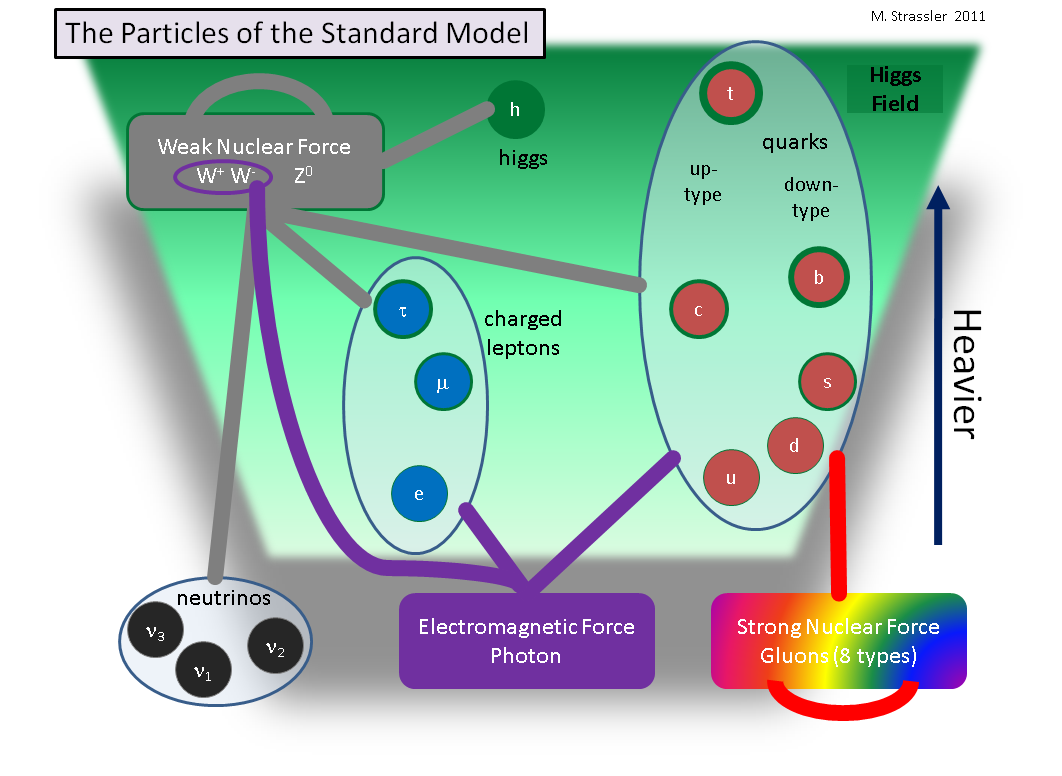
\includegraphics[width=0.80\textwidth]{sm_interactions2}
    \caption[SM particles and force carriers]{SM particles and force carriers. Self-interactions are also shown. The strength of the coupling to the Higgs boson increases from the bottom to the top, which is illustrated by the shades of the green color (the Higgs field).  }
    \label{sm_interactions2}
\end{figure}


The third and, arguably the most important stage, is the Higgs boson. The Higgs boson is the excitation of the BEH field. Thus, the Higgs bosons can be produced at colliders by pumping more and more energy in a small space-time region exciting the BEH field to ``produce'' the Higgs bosons. In reality this happens through making the LHC beams more energetic and thus, during the collision, producing more energetic gluons (and also more energetic quarks). The main Higgs boson production mechanism is called gluon fusion. During this process, two gluons interact through the virtual top quark loop and a Higgs boson is produced as a result. This accounts for about $90\%$ of the overall LHC Higgs production at the 13 TeV energy. The second mechanism is vector boson fusion. The third mechanism is associated production with a weak boson. The smallest contributor to the Higgs boson production is the $t\bar{t}H$ process, which stands for the associated production of the top anti-top quark pair with the Higgs boson. All mentioned Higgs boson production mechanisms are presented in the form of Feynman diagrams in Fig. \ref{higgs_production}. The plot at the bottom is for the 8 TeV centre-of-mass energy. At 13 TeV the exact numbers for curves are different, but the main trends remain. 


\begin{figure}[H]
  \centering
    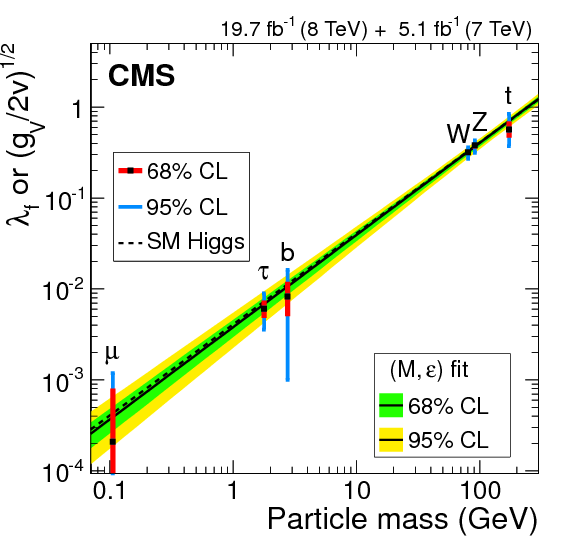
\includegraphics[width=0.80\textwidth]{coupling_ff} %_copy
    \caption[Coupling of particles to SM Higgs boson]{Coupling of particles to SM Higgs boson versus the mass of the particle, log-log scale is used. The y axis accommodates the couplings for both fermions and bosons. }
    \label{coupling_ff}
\end{figure}





\begin{figure}[H]
  \centering
\hspace{1cm}    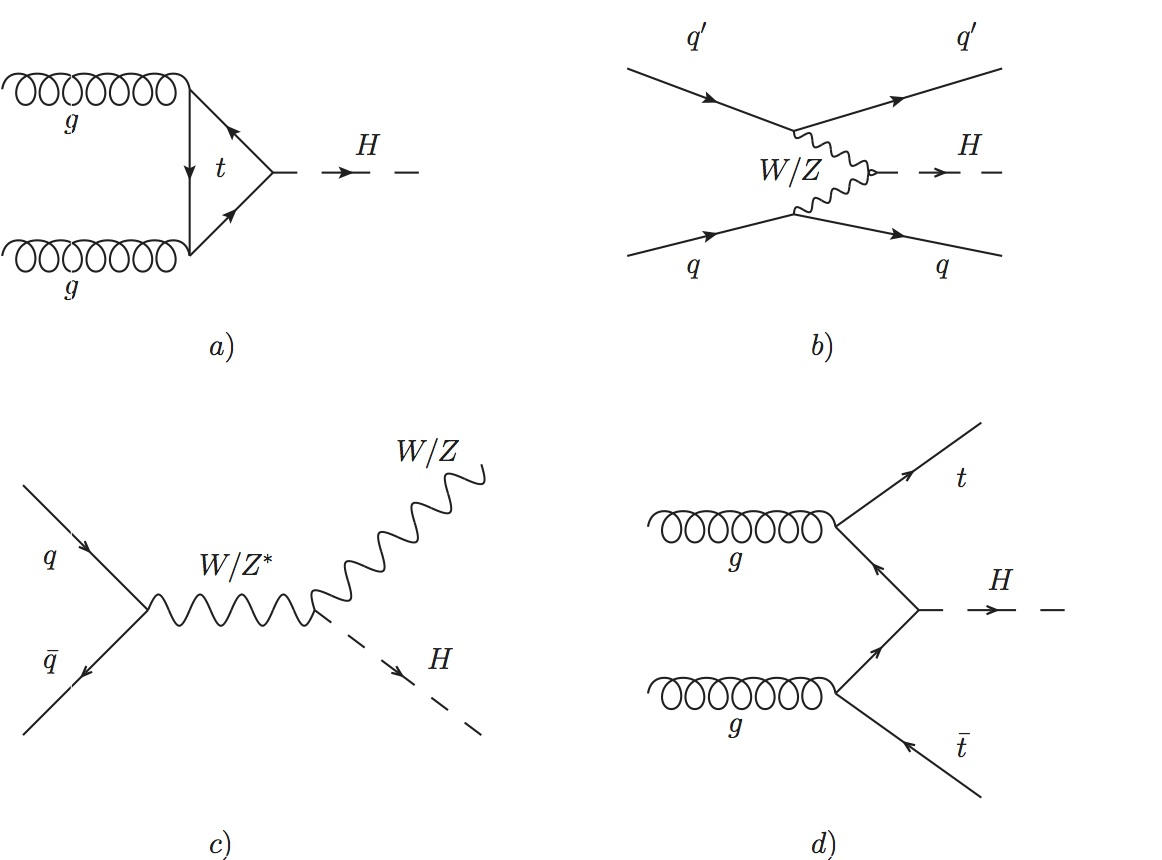
\includegraphics[width=0.8\textwidth]{higgs_production}\\
    \vspace{1cm}
       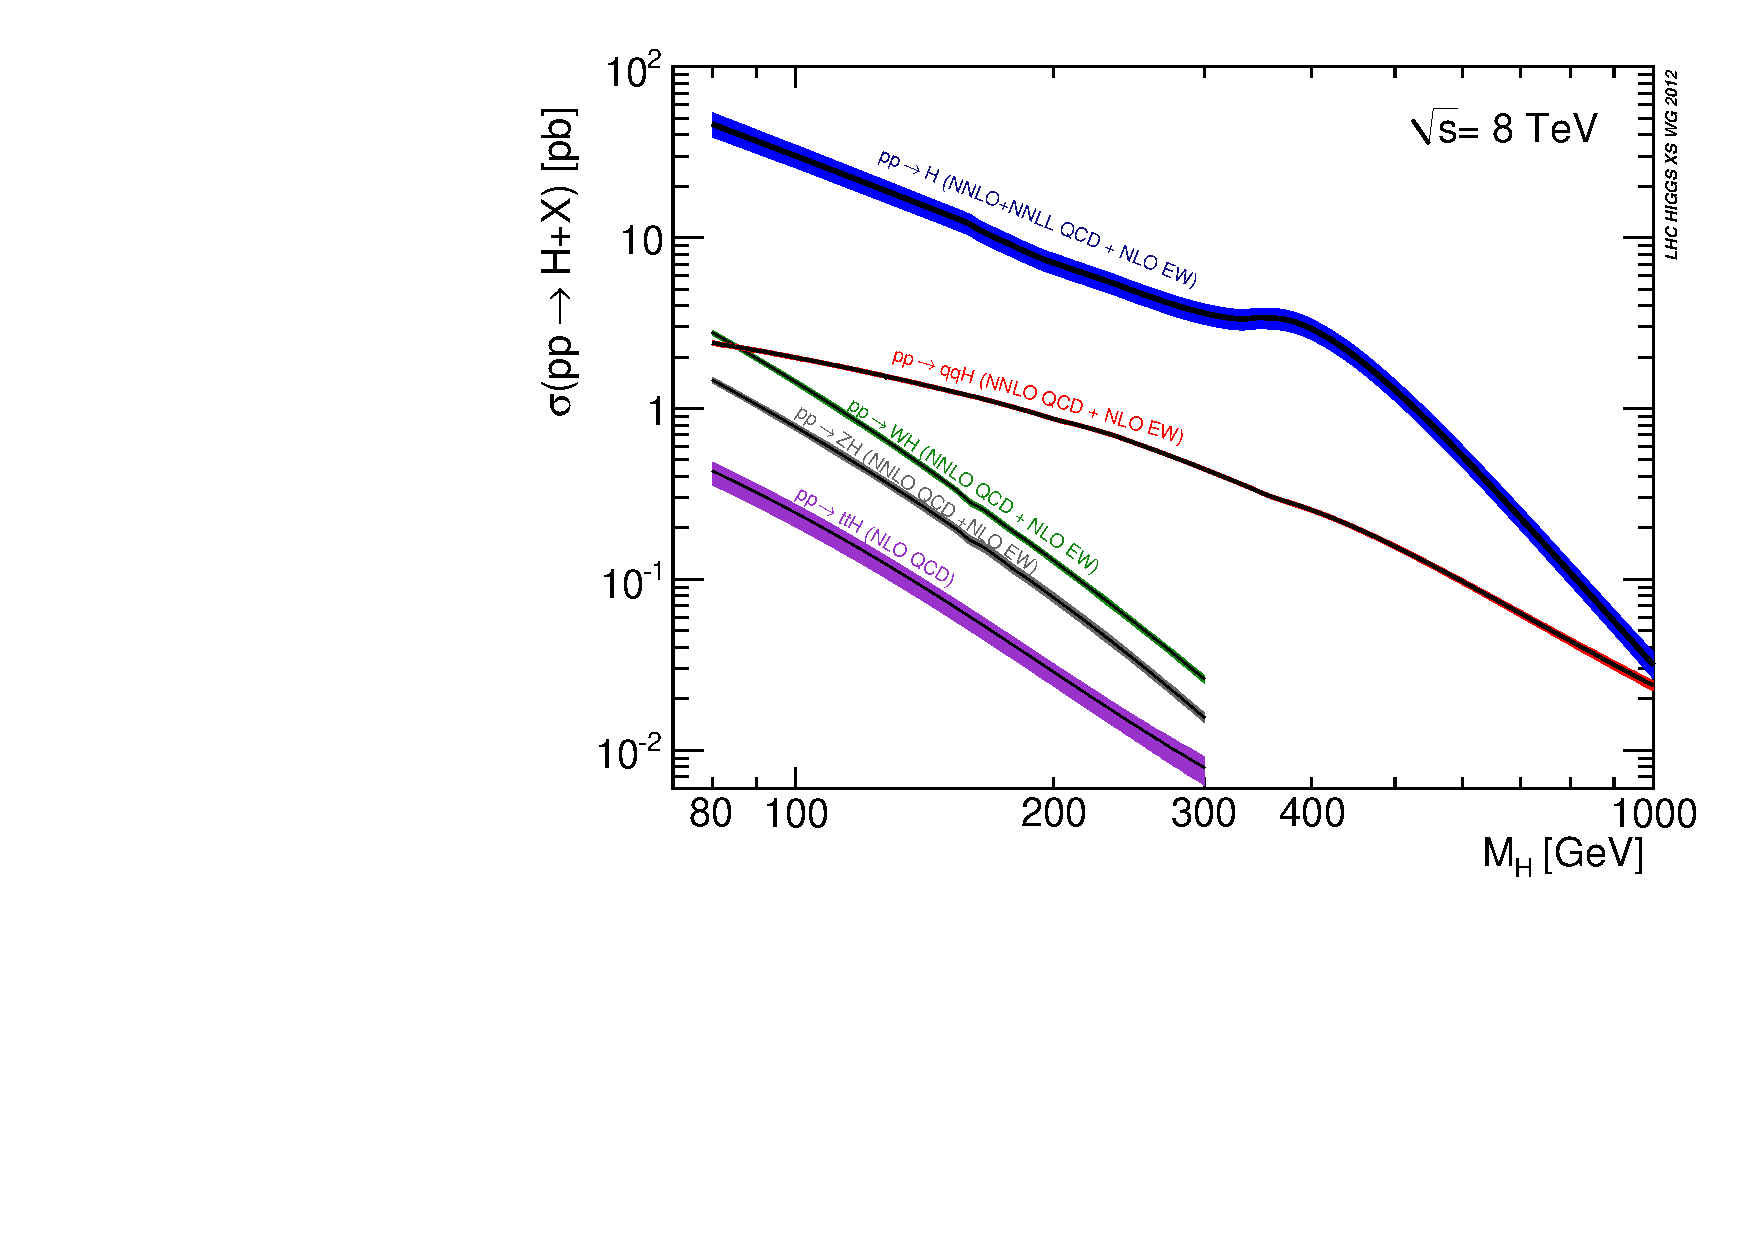
\includegraphics[width=0.7\textwidth]{Higgs_XS_8TeV_lx.pdf}
    \caption[SM Higgs boson production modes]{Top: SM Higgs boson production modes: a) a gluon fashion (in blue color at the bottom), b) a vector boson scattering (red),  c) an associated production with a vector boson (green and brown), d) an associated production with the top anti-top pair (purple). Bottom: Higgs boson production modes as a function of the Higgs boson mass. }
    \label{higgs_production}
\end{figure}


When describing Higgs boson physics one cannot avoid mentioning the decay channels of the Higgs boson. In physics, the term ``branching fraction'' is used to quantify the probabilities with which a parent particle decays to daughter particles (see Fig. \ref{Higgs_BR_LM_RECT}). The picture shows a classic plot produced by theorist before the Higgs boson discovery in 2012. The values of branching fractions are given as a function of the Higgs boson mass. In this thesis we work with the SM Higgs bosons ($\approx $125 GeV) and the measurement focuses on two specific Higgs boson decays, $H\to b\bar{b}$ and $H\to ZZ$. The first one has the highest branching fraction, while the second one gives a clean signature when subsequent $Z \to \ell\ell$ decays are selected. 

Before we conclude with the BEHGHK method, a little bit of history, an irony of life, actually. The BEH particle is called the Higgs boson, but Peter Higgs was not the first to publish the article on the BEH mechanism, in fact, he was the last of the BEHGHK authors. His very first article was rejected since it contained no specific predictions or conclusions drawn from his calculations. This is why he was out-published by others. But this rejection made him write another article where he explicitly predicted the existence of the new boson. This is what made all the difference, as he was the first to predict a new boson, and so this boson now is called the Higgs boson. 

\begin{figure}[H]
  \centering
    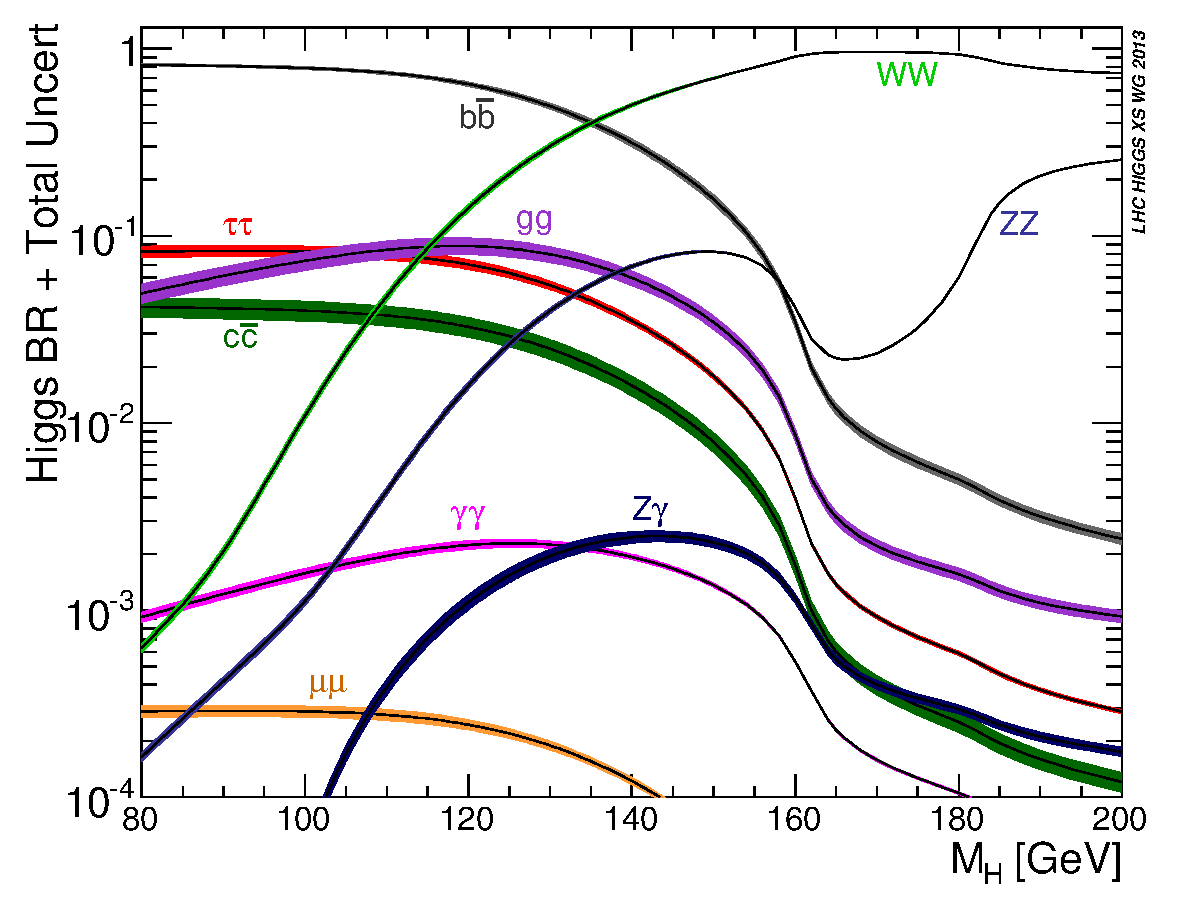
\includegraphics[width=0.75\textwidth]{Higgs_BR_LM_RECT}
    \caption[Higgs boson decay channels]{Higgs boson decay channels as a function of the Higgs boson mass. At 125 GeV the dominant decay mode is $H \to b\bar{b}$.}
    \label{Higgs_BR_LM_RECT}
\end{figure}






Even though the facts above tell us about how great the SM is, the SM is still far from being perfect. Masses of elementary particles are the parameters in this theory; they do not come from SM predictions. It is hypothesized that the SM could be a part of the larger ultimate theory, the so-called ``Theory of Everything'' (TOE), which is yet to be written (and was a dream of another genius, Einstein \cite{aps_einstein}). There is hope that the TOE will be able to explain many phenomena, such as the quark mass hierarchy, flavor mixing, etc. Also, in the SM all neutrinos are massless; however, it has been shown that they have a non-zero mass \cite{Bilenky:2014ema}. This fact is one of the main motivations for physicists to look for extensions of the SM. 



